
% Environments for repeating propositions.
\newtheorem*{propAngle}{Proposition \ref{prop:angle}}
\newtheorem*{propAngle:b}{Proposition \ref{prop:angle:b}}
\newtheorem*{propIV}{Proposition \ref{prop:IV}}
\newtheorem*{propkappa}{Proposition \ref{prop:kappa}}
\newtheorem*{propIVb}{Proposition \ref{prop:IV:b}}


\begin{figure}[t]
\begin{center}
\begin{tabular}{cc}
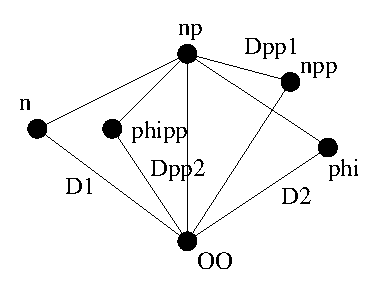
\includegraphics[width=1.2in]{images/phiTriangles.eps} \quad &
\quad
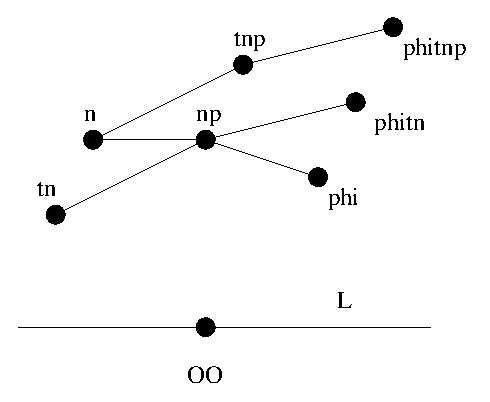
\includegraphics[width=1.2in]{images/phiDiff2.eps} \\
(a) & (b)
\end{tabular}
\end{center}
\caption{
(a) Triangles $\Delta_1$, $\Delta_2$, $\Delta''_1$ and $\Delta''_2$.
(b) Rotating $n$ and $\tn'$ around line $L$.}
\label{fig:triangles}
\end{figure}

\section{Proofs}

\subsection{Angle Lemmas}

Let $n$ and $n'$ be unit vectors in $\Rthree$.
Recall the following definitions, from Section~\ref{sec:reliable}.
\begin{align*}
\Orth(n,n') & = n - (n \cdot n') n' \\ 
\phi(n,n') & = n - 2 \times \Orth(n,n') = 2(n \cdot n') n' - n.
\end{align*}
Vector $\Orth(n,n')$ is the component of $n$ orthogonal to $n$.
Vector $\phi(n,n')$ is the vector 
{\em predicted by} $n$ and $n'$.

\begin{align*}
\cos(\angle(\phi(n,n'),n')) & = (2 (n \cdot n') n' -n) \cdot n' \\
  & = 2 (n \cdot n') (n' \cdot n') - (n \cdot n') \\
  & = 2 (n \cdot n') - (n \cdot n') \mbox{  (since $n'$ is a unit vector)} \\
  & = n \cdot n' = \cos(\angle(n,n')).
\end{align*}
Thus, $\angle(\phi(n,n'),n')$ equals $\angle(n,n')$.

\begin{lemma}
If $n$, $n'$ and $n''$ are unit vectors, then
\begin{enumerate}
\item $\Lambda(n,n',n'') = \Lambda(n'',n',n)$, and
\item $\angle(n,n'') = \angle(\phi(n,n'),\phi(n'',n'))$.
\end{enumerate}
\label{lemma:phi}
\end{lemma}

\begin{proof}
Let $\OO$ be the origin $(0,0,0)$.
Let $\Delta_1$, $\Delta_2$, $\Delta''_1$ and $\Delta''_2$
be the triangles $\Delta(\OO,n',n)$, $\Delta(\OO,n',\phi(n,n'))$,
$\Delta(\OO,n',n'')$ and $\Delta(\OO,n',\phi(n'',n'))$, respectively.
(See Figure~\ref{fig:triangles}.(a).)

As noted above, $\angle(n,n')$ equals $\angle(\phi(n,n'),n')$.
Similarly, $\angle(n',n'')$ equals $\angle(\phi(n'',n'), n')$.
Since $n$, $n'$ and  $\phi(n,n')$ have the same (unit) length,
triangles $\Delta_1$ and $\Delta_2$ are congruent.
Since $n'$, $n''$ and  $\phi(n'',n')$ have the same (unit) length,
triangles $\Delta''_1$ and $\Delta''_2$ are congruent.

Since $n$, $n'$ and $\phi(n,n')$ are co-planar
and $n''$, $n'$ and $\phi(n'',n')$ are co-planar,
the dihedral angles between $\Delta_1$ and $\Delta''_2$ 
equals the dihedral angle between $\Delta_2$ and $\Delta''_1$.
Thus, tetrahedron $(\OO,n,n',\phi(n'',n'))$ is congruent
to tetrahedron $(\OO,n',n'',\phi(n,n'))$
and $\angle(n, \phi(n'',n'))$ equals $\angle(n'', \phi(n,n'))$
and $\angle(n,n'')$ equals $\angle(\phi(n,n'),\phi(n'',n'))$.
\end{proof}

The following corollary describes how $\angle(\phi(n,n'))$
and $\Lambda(n,n',n'')$ change when unit vector $n$ is replaced by $\tn$.
\begin{corollary}
If $n$, $\tn$, $n'$ and $n''$ are unit vectors
and $\angle(n,\tn) \le \mu$, then
\begin{enumerate}
\item $\angle(\phi(n,n'),\phi(\tn,n')) \le \mu$;
\item $|\Lambda(n,n',n'') - \Lambda(\tn,n',n'')| \le \mu$.
\end{enumerate}
\label{corollary:phi}
\end{corollary}

\begin{proof}
By Lemma~\ref{lemma:phi},
angle $\angle(n,\tn)$ equals $\angle(\phi(n,n'), \phi(\tn,n'))$.
(Let $n''$ represent $\tn$ in Lemma~\ref{lemma:phi}.)
Thus,
\begin{align*}
\angle(\phi(n,n'),\phi(\tn,n')) & = \angle(n,\tn) \le \mu, \qquad \mbox{and} \\
|\Lambda(n,n',n'') - \Lambda(\tn,n',n'')| & = 
|\angle(\phi(n,n'),n'') - \angle(\phi(\tn,n'),n'')|  \\
  & \le \angle(\phi(n,n'),\phi(\tn,n')) \le \mu.
\end{align*}
\end{proof}

In the following corollary,
vector $n'$ is replaced by $\tn'$.
The bounds are slightly different than the bounds in the previous corollary.
\begin{corollary}
If $n$, $n'$, $\tn'$, $n''$ and $n'''$ are unit vectors
and $\angle(n',\tn') \le \mu$ and $\angle(\phi(n,n'),n'') \le \gamma$, 
then
\begin{enumerate}
\item $\angle(\phi(n,n'),\phi(n,\tn')) \le 2\mu$;
\item $|\Lambda(n,n',n'') - \Lambda(n,\tn',n'')| \le 2\mu$;
\item $|\Lambda(n',n'',n''') - \Lambda(n',\phi(n,n'),n''') \le 2\gamma$.
\end{enumerate}
\label{corollary:phi:2}
\end{corollary}

\begin{proof}
Let $L$ be the line through the origin orthogonal to $n'$ and $\tn'$.
Rotating $\tn'$ and $n$ by angle $\angle(\tn',n')$ around $L$
maps $\tn'$ to $n'$ and $n$ to a unit vector $\tn$
where $\angle(n,\tn) \le \mu$ (Figure~\ref{fig:triangles}.(b).)
By Corollary~\ref{corollary:phi},
$\angle(\phi(n,n'),\phi(\tn,n')) \le \mu$.
Rotating $\tn$, $n'$ and $\phi(\tn,n')$ by angle $-\angle(\tn',n')$ around $L$
maps $\tn$ back to $n$, vector $n'$ to $\tn'$ and $\phi(\tn,n')$
to $\phi(n,\tn')$.
Since $|-\angle(\tn',n')| \le \mu$,
angle $\angle(\phi(\tn,n'),\phi(n,\tn')) \le \mu$.
Thus,
\begin{align*}
\angle(\phi(n,n'),\phi(n,\tn')) 
 & \le \angle(\phi(n,n'),\phi(\tn,n')) + \angle(\phi(\tn,n'),\phi(n,\tn')) \\
 & \le 2 \mu,
\end{align*}
and
\begin{align*}
|\Lambda(n,n',n'') - \Lambda(n,\tn',n'')| & = 
|\angle(n'', \phi(n,n')) - \angle(n'', \phi(n,\tn'))|  \\
  & \le \angle(\phi(n,n'),\phi(n,\tn')) \le 2\mu.
\end{align*}

Replacing $n$, $n'$, $\tn'$, $n''$ and $\mu$
by $n'$, $n''$, $\phi(n,n')$, $n'''$ and $\gamma$ in the formula above,
gives
\begin{align*}
|\Lambda(n',n'',n''') - \Lambda(n',\phi(n,n'),n''')| \le 2 \gamma.
\end{align*}

\end{proof}

\begin{lemma}
If $n$, $n'$ and $n''$ are unit vectors, then
\begin{enumerate}
\item $\phi_2(n,n') = \phi_1(n',\phi_1(n,n')$, and
\item $\Lambda_2(n,n',n'') = \Lambda_1(n', \phi_1(n,n'), n''))$.
\end{enumerate}
\label{lemma:Lambda2}
\end{lemma}

\begin{proof}

By definition,
\begin{align*}
\phi_2(n,n') = \phi_1(\phi_0(n,n'), \phi_1(n,n')) = \phi_1(n', \phi_1(n,n')).
\end{align*}

Thus,
\begin{align*}
\Lambda_2(n,n',n'') & = \angle(\phi_2(n,n'),n'') \\
  & = \angle(\phi_1(n',\phi_1(n,n')), n'')  
    = \Lambda_1(n', \phi_1(n,n'), n'').
\end{align*}

\end{proof}

\begin{corollary}
If $n$, $n'$ and $n''$ are unit vectors
and $\angle(n,\tn) \le \mu$,
then $|\Lambda_2(n,n',n'') - \Lambda_2(\tn,n',n'')| \le 2\mu$.
\label{corollary:Lambda2}
\end{corollary}

\begin{proof}

By Lemma~\ref{lemma:phi},
\begin{align*}
\angle(\phi_1(n,n'),\phi_1(\tn,n')) = \angle(n,\tn) \le \mu.
\end{align*}

Thus,
\begin{align*}
\Lambda_2(n,n',n'') & = \Lambda_1(n', \phi(n,n'), n'') 
  & \mbox{(Lemma~\ref{lemma:Lambda2})} \\
& \le \Lambda_1(n', \phi(\tn,n'), n'') + 2\mu
  & \mbox{(Corollary~\ref{corollary:phi:2})} \\
& = \Lambda_2(\tn,n',n'') + 2 \mu.
\end{align*}

Swapping $n$ and $\tn$ gives
$\Lambda_2(\tn,n',n'') \le \Lambda_2(n, n',n'') + 2 \mu$.
Thus,
$|\Lambda_2(n,n',n'') - \Lambda_2(\tn, n',n'')| \le 2 \mu$.
\end{proof}

\begin{corollary}
If $n$, $n'$ and $n''$ are unit vectors
and $\angle(n',\tn') \le \mu$,
then $|\Lambda_2(n,n',n'') - \Lambda_2(n,\tn',n'')| \le 3\mu$.
\label{corollary:Lambda2:2}
\end{corollary}

\begin{proof}

By Lemma~\ref{lemma:phi},
\begin{align*}
\angle(\phi_1(n,n'),\phi_1(n,\tn')) = \angle(n',\tn') \le \mu.
\end{align*}

Thus,
\begin{align*}
\Lambda_2(n,n',n'') & = \Lambda_1(n', \phi(n,n'), n'') 
  & \mbox{(Lemma~\ref{lemma:Lambda2})} \\
& \le \Lambda_1(\tn', \phi(n,n'), n'') + \mu
  & \mbox{(Corollary~\ref{corollary:Lambda2})} \\
& \le \Lambda_1(\tn', \phi(n,\tn'), n'') + 2\mu + \mu
  & \mbox{(Corollary~\ref{corollary:phi:2})} \\
& = \Lambda_2(n,\tn',n'') + 3 \mu.
\end{align*}

Swapping $n'$ and $\tn'$ gives
$\Lambda_2(n,n',n'') \le \Lambda_2(n, \tn',n'') + 3 \mu$.
Thus,
$|\Lambda_2(n,\tn',n'') - \Lambda_2(n, \tn',n'')| \le 3 \mu$.

\end{proof}

\begin{corollary}
If $n$, $n'$, $n''$ and $n'''$ are unit vectors
and $\Lambda(n,n',n'') \le \gamma$
and $\Lambda(n',n'',n''') \le \gamma$,
then $\Lambda_2(n,n',n''') \le 3\gamma$.
\label{corollary:Lambda2:3}
\end{corollary}

\begin{proof}
By assumption, $\Lambda_1(n,n',n'') \le \gamma$,
so $\angle(\phi_1(n,n'),n'') \le \gamma$.
\begin{align*}
\Lambda_2(n,n',n''') & = \Lambda_1(n', \phi_1(n,n'), n'')
 & \mbox{(Lemma~\ref{lemma:Lambda2})} \\
 & \le \Lambda_1(n', n'', n''') + 2 \gamma 
 & \mbox{(Corollary~\ref{corollary:phi:2})} \\
 & \le 3\gamma.
\end{align*}
\end{proof}


\subsection{Angle bounds}

We now give bounds on $\Lambda$ and on the angles
between the exact and approximated normals.

\begin{propAngle}
Let $(v, v', v'')$ be a collinear sequence of adjacent vertices
contained in $A_i$ for some smooth region $A_i$.
\begin{enumerate}
\item If $v, v', v'' \in \IV(A_i)$, then\\
{\centering
$\Lambda(\tn_v, \tn_{v'}, \tn_{v''}) \le 
\Lambda(n_v, n_{v'}, n_{v''}) + 4 \mu \le \lambda + 4 \mu$.}
\item If $v, v' \in \IV(A_i)$, then
$\angle(n_{v''},\tn_{v''}) \le 
   \Lambda(\tn_v,\tn_{v'},\tn_{v''}) + 3 \mu + \lambda$.
\end{enumerate}
\end{propAngle}

\begin{proof}[Proof of \ref{prop:angle}.1]
Since $v$, $v'$ and $v''$ are interior vertices,
angles $\angle(n_v,\tn_v)$, $\angle(n_{v'}, \tn_{v'})$ 
and $\angle(n_{v''}, \tn_{v''})$ are all less than $\mu$.
\begin{align*}
\Lambda(\tn_v,\tn_{v'},\tn_{v''}) & \le \Lambda(\tn_v, \tn_{v'}, n_{v''}) + \mu 
    \\
  & \le \Lambda(n_v, \tn_{v'}, n_{v''}) + \mu + \mu 
    & \mbox{(Corollary~\ref{corollary:phi})} \\
  & \le \Lambda(n_v, n_{v'}, n_{v''}) + 2\mu + \mu + \mu 
    & \mbox{(Corollary~\ref{corollary:phi:2})} \\
  & = \Lambda(n_v, n_{v'}, n_{v''}) + 4 \mu \le \lambda + 4 \mu.
\end{align*}

\end{proof}

\begin{proof}[Proof of \ref{prop:angle}.2]

\begin{align*}
\angle(n_{v''},\tn_{v''}) & \le \angle(\phi(n_v,n_{v'}),n_{v''}) +
\angle(\phi(n_v,n_{v'}),\tn_{v''}) \\
& \le \lambda + \Lambda(n_v, n_{v'}, \tn_{v''}).
\end{align*}

Since $\angle(n_v,\tn_v) \le \mu$,
\begin{align*}
\Lambda(n_v, n_{v'}, \tn_{v''}) & 
  \le \Lambda(\tn_v, n_{v'}, \tn_{v''}) + \mu.
& \mbox{(Corollary~\ref{corollary:phi})}
\end{align*}

Since $\angle(n_{v'},\tn_{v'}) \le \mu$,
\begin{align*}
\Lambda(\tn_v, n_{v'}, \tn_{v''}) & 
\le \Lambda(\tn_v, \tn_{v'}, \tn_{v''}) + 2\mu.
& \mbox{(Corollary~\ref{corollary:phi:2})}
\end{align*}

Thus,
\begin{align*}
\Lambda(n_v, n_{v'}, \tn_{v''}) & \le \Lambda(\tn_v, n_{v'}, \tn_{v''}) + \mu
\le \Lambda(\tn_v, \tn_{v'}, \tn_{v''}) + 3\mu, \mbox{ and} \\
\angle(n_{v''},\tn_{v''}) & \le \lambda + \Lambda(n_v, n_{v'}, \tn_{v''})
  \le \lambda + \Lambda(\tn_v, \tn_{v'}, \tn_{v''}) + 3\mu \\
& = \Lambda(\tn_v, \tn_{v'}, \tn_{v''}) + 3\mu+ \lambda.
\end{align*}

\end{proof}

The following corollary follows directly from Proposition~\ref{prop:angle}.1.
\begin{corollary}
Let $(v,v',v'')$ be a collinear sequence of adjacent grid vertices
where vertices $v,v',v'' \in A_1$
and $v'$ and $v''$ are interior vertices in $A_1$.
If $\Lambda(\tn_v,\tn_{v'},\tn_{v''}) \le \alpha$, then
\begin{equation*}
\angle(n_{v''},\tn_{v''}) \le \alpha + 3 \mu + \lambda.
\end{equation*}
\label{corollary:collinear}
\end{corollary}

The proofs of Proposition~\ref{prop:angle:b} are similar
to the proofs of Proposition~\ref{prop:angle}.

\begin{propAngle:b}
Let $(v, v', v'',v''')$ be a collinear sequence of adjacent vertices
contained in $A_i$ for some smooth region $A_i$.
\begin{enumerate}
\item If $v, v', v'', v''' \in \IV(A_i)$, then\\
{\centering
$\Lambda_2(\tn_v, \tn_{v'}, \tn_{v'''}) \le 
\Lambda_2(n_v, n_{v'}, n_{v'''}) + 4 \mu \le 3\lambda + 6 \mu$.}
\item If $v, v' \in \IV(A_i)$, then\\
{\centering
$\angle(n_{v'''},\tn_{v'''}) 
   \le \Lambda(\tn_v,\tn_{v'},\tn_{v'''}) + 3\lambda+ 5 \mu$.}
\end{enumerate}
\end{propAngle:b}

\begin{proof}[Proof of~\ref{prop:angle:b}.1]

Since $v$, $v'$, $v''$ and $v'''$ are interior vertices,
angles $\angle(n_v,\tn_v)$, $\angle(n_{v'}, \tn_{v'})$,
$\angle(n_{v''}, \tn_{v''})$ and $\angle(n_{v'''},\tn_{v'''})$
are all less than $\mu$.
\begin{align*}
\Lambda_2(\tn_v,\tn_{v'},\tn_{v'''}) 
  & \le \Lambda_2(\tn_v, \tn_{v'}, n_{v'''}) + \mu \\
  & \le \Lambda_2(n_v, \tn_{v'}, n_{v'''}) + \mu + 2\mu 
    & \mbox{(Corollary~\ref{corollary:Lambda2})} \\
  & \le \Lambda_2(n_v, n_{v'}, n_{v'''}) + 3\mu + 2\mu + \mu 
    & \mbox{(Corollary~\ref{corollary:Lambda2:2})} \\
  & = \Lambda_2(n_v, n_{v'}, n_{v'''}) + 6 \mu \\
  & \le 3\lambda +  6 \mu.  
    & \mbox{(Corollary~\ref{corollary:Lambda2:3})}
\end{align*}

\end{proof}

\begin{proof}[Proof of~\ref{prop:angle:b}.2]

\begin{align*}
\angle(n_{v'''},\tn_{v'''}) 
  &  \le \angle(\phi_2(n_v, n_{v'}), n_{v'''}) 
         + \angle(\phi_2(n_v,n_{v'}), \tn_{v'''}) \\
  & = \Lambda_2(n_v, n_{v'}, n_{v'''}) 
      + \angle(\phi_2(n_v,n_{v'}), \tn_{v'''}) \\
  & \le 3 \lambda + \Lambda_2(n_v, n_{v'}, \tn_{v'''}).
  & \mbox{(Lemma~\ref{lemma:Lambda2})}
\end{align*}

Since $\angle(n_v,\tn_v) \le \mu$,
\begin{align*}
\Lambda_2(n_v, n_{v'}, \tn_{v'''}) 
  & \le \Lambda_2(\tn_v, n_{v'}, \tn_{v'''}) + 2\mu.
& \mbox{(Corollary~\ref{corollary:Lambda2})}
\end{align*}

Since $\angle(n_{v'},\tn_{v'}) \le \mu$,
\begin{align*}
\Lambda_2(\tn_v, n_{v'}, \tn_{v'''}) & 
\le \Lambda_2(\tn_v, \tn_{v'}, \tn_{v'''}) + 3\mu.
& \mbox{(Corollary~\ref{corollary:Lambda2:2})}
\end{align*}

Thus,
\begin{align*}
\Lambda_2(n_v, n_{v'}, \tn_{v'''}) 
   & \le \Lambda_2(\tn_v, n_{v'}, \tn_{v'''}) + 2\mu
\le \Lambda_2(\tn_v, \tn_{v'}, \tn_{v'''}) + 5\mu, \mbox{ and} \\
\angle(n_{v'''},\tn_{v'''}) & \le 3\lambda + \Lambda_2(n_v, n_{v'}, \tn_{v'''})
  \le 3\lambda + \Lambda_2(\tn_v, \tn_{v'}, \tn_{v'''}) + 5\mu \\
& = \Lambda_2(\tn_v, \tn_{v'}, \tn_{v'''}) + 3\lambda + 5 \mu.
\end{align*}

\end{proof}


We also give bounds on $\angle(\tn_v, \tn_{v'})$
and on  $\angle(n_{v'},\tn_{v'})$.
We first define a bound $\kappa$ on $\angle(n_v,n_{v'})$
in smooth regions of $f$.
\begin{align*}
\kappa = \max\{ \angle(n_v,n_{v'}) v,v' \in A_i \mbox{ for some } A_i \}.
\end{align*}
Value $\kappa$ can be viewed as a bound on the curvature of the field
within smooth regions.
In comparison, $\lambda$ is a bound on the change in curvature
of the field within smooth regions.

The following proposition gives bounds on $\angle(n_{v'},\tn_{v'})$
based on $\angle(\tn_v, \tn_{v'})$.
\begin{proposition}
Let $v$ and $v'$ be adjacent vertices contained in $A_i$
for some smooth region $A_i$.
\begin{enumerate}
\item If $v, v' \in \IV(A_i)$, then
$\angle(\tn_v, \tn_{v'}) \le \angle(n_v, \tn_{v'}) + 2 \mu \le \kappa + 2 \mu$.
\item If $v \in \IV(A_i)$, then
$\angle(n_{v'}, \tn_{v'}) \le \angle(\tn_v, \tn_{v'}) + \kappa + \mu$.
\end{enumerate}
\label{prop:kappa}
\end{proposition}

\begin{proof}[Proof of \ref{prop:kappa}.1.]
\begin{align*}
\angle(\tn_v,\tn_{v'}) & \le \angle(n_v, \tn_{v'}) + \angle(n_v, \tn_v)
              \le \angle(n_v, \tn_{v'}) + \mu \\
             & \le \angle(n_v, n_{v'}) + \angle(n_{v'}, \tn_{v'}) + \mu \\
             & \le \angle(n_v, n_{v'}) + \mu + \mu 
               = \angle(n_v,n_{v'}) + 2 \mu \le \kappa+ 2 \mu.
\end{align*}
\end{proof}


\begin{proof}[Proof of \ref{prop:kappa}.2.]
\begin{align*}
\angle(n_{v'},\tn_{v'}) & \le \angle(n_v,\tn_{v'}) + \angle(n_v, n_{v'})
  \le \angle(n_v,\tn_{v'}) + \kappa \\
& \le \angle(\tn_v, \tn_{v'}) + \angle(n_v,\tn_v) + \kappa
  \le \angle(\tn_v, \tn_{v'}) + \mu + \kappa.
\end{align*}
\end{proof}

\subsection{Containment bounds}

To prove Proposition~\ref{prop:IV},
we show that if a sufficiently large ball $\BB$ contains vertex $v$,
then $\BB$ contains $N(v'')$ and $N(v''')$
for some collinear sequence $(v,v',v'',v''')$.
\begin{lemma}
Let $\Gamma$ be a regular grid whose edges all have the same length $L$.
If some ball $\BB$ of radius $(5/2) \sqrt{3}L$ contains grid vertex $v$,
then there is a collinear sequence $(v,v',v'',v''')$ 
of adjacent grid vertices
such that $\BB$ contains $N(v'')$ and $N(v''')$.
\label{lemma:ball}
\end{lemma}

\begin{proof}
Let $\BB$ be a ball of radius $(5/2)\sqrt{3}L$ containing grid vertex $v$.
Let $q$ be the center of $\BB$.
Without loss of generality assume vertex $v$ is at the origin $(0,0,0)$,
that the edge length $L$ equals 1,
and that $q$ lies in the positive $x$, $y$ and $z$ orthant.
Let $D \le (5/2) \sqrt{3}$ be the distance from the origin to $q$.
The coordinates of $q$ can be expressed as $D(u_x,u_y,u_z)$
where $(u_x,u_y,u_z)$ is a unit vector.

Without loss of generality, assume that $q$ is closest to the $x$-axis,
i.e., $u_x \ge u_y$ and $u_x \ge u_z$.
Let $v''$ be $(2,0,0)$ and $v'''$ be $(3,0,0)$.
We claim that $N_{v''}$ and $N_{v'''}$ are in $\BB$.

Let $p$ be the grid vertex with coordinates $(3,-1,0)$.
Point $p$ is in $N_{v''}$.
Let $R$ equal $(5/2)\sqrt{3}$.
Since ball $\BB$ contains the origin,
distance $D$ is at most $R$.
\begin{align*}
|q-p|^2 & = (D u_x-3)^2 + (D u_y+1)^2 + (D u_z)^2 \\
 & = D^2 u_x^2 - 6 D u_x + 9 + D^2 u_y^2 + 2 D u_y + 1 + D^2 u_z^2 \\
 & = D^2 (u_x^2 + u_y^2 + u_z^2) + 10 - 6 D u_x + 2 D u_y \\
 & = D^2 + 10 - 6 D u_x + 2 D u_y \\
 & \le D^2 + 10 - 4 D u_x \mbox{  (since $u_y \le u_x$)} \\
 & = (R + D-R)^2 +10 - 4 (R + D-R) u_x \\
 & = R^2 + 2R(D-R) + (D-R)^2 + 10 - 4R u_x - 4 (D-R) u_x \\
 & = R^2 + (10 - 4R u_x) + (D-R)(2R + D-R - 4 u_x) \\
 & = R^2 + (10 - 4R u_x) - (R-D) (D+R - 4 u_x).
\end{align*}

Since $u_x \ge u_y$ and $u_x \ge u_z$, 
coordinate $u_x$ is at least $1/\sqrt{3}$.
\begin{align*}
10 - 4 Ru_x & = 10 - 4 (5/2) \sqrt{3} u_x \\
 & \le 10 - 10 \sqrt{3} (1/\sqrt{3}) \mbox{ since $u_x \ge 1/\sqrt{3}$} \\
 & = 10 - 10 = 0.
\end{align*}

\begin{align*}
D + R - 4u_x & \ge R - 4 = (5/2)\sqrt{3} - 4 \ge 4.3 - 4 > 0.
\end{align*}

Since $\BB$ contains the origin,
distance $D$ is at most $R$ and $(R-D) \ge 0$.
Thus,
\begin{align*}
|q-p|^2 & = R^2 + (10 - 4R u_x) - (R-D) (D+R - 4 u_x) \\
   & \le R^2 + 0 - (R-D) (D+R - 4 u_x) \mbox{  (since $(10-4Ru_x) \le 0$)} \\
   & \le R^2 \mbox{  (since $(R-D)>0$ and $(D+R-4u_x)>0$.)}
\end{align*}
so $\BB$ contains $(3,-1,0)$.

A similar analysis shows that $\BB$ contains $(3,0,-1)$,
$(3,1,0)$, $(3,0,1)$, $(2,0,0)$ and $(4,0,0)$.
Thus, $\BB$ contains $N(v''')$.

A similar analysis shows that $\BB$ contains $N(v'')$.
\end{proof}
The bound $(5/2) \sqrt{3} L$ is tight.
If we place a ball $\BB$ of radius $(2.5-\epsilon) \sqrt{3}L$ at 
the point $(2.5-\epsilon,2.5-\epsilon,2.5-\epsilon)L$,
then ball $\BB$ contains the origin.
However, ball $\BB$ does not contain $N(v'')$ or $N(v''')$
for any collinear sequence $(v,v',v'',v''')$.

As before, $\XX = \cup_{A_j} \partial A_j$ is the union of all the boundaries
of smooth regions $A_j$.
Proposition~\ref{prop:IV} follows directly from Lemma~\ref{lemma:ball}.
\begin{propIV}
Let $\Gamma$ be a regular grid whose edges all have the same length $L$.
If some ball $\BB$ of radius $(5/2)\sqrt{3}L$ contains grid vertex $v \in A_i$
and does not intersect $\XX$,
then there is a collinear sequence $(v,v',v'',v''')$ 
of adjacent grid vertices 
such that $v'' \in \IV(A_i)$ and $v''' \in \IV(A_i)$.
\end{propIV}

\begin{proof}
By Lemma~\ref{lemma:ball}, ball $\BB$ contains $N(v'')$ and $N(v''')$
for some collinear sequence $(v,v',v'',v''')$.
Since ball $\BB$ does not intersect $\XX$,
\begin{align*}
N(v'') & \subseteq \BB \subseteq A_i, \mbox{  and} \\
N(v''') & \subseteq \BB \subseteq A_i.
\end{align*}
Thus, $v'' \in \IV(A_i)$ and $v''' \in IV(A_i)$.
\end{proof}

We can also give a reformulation of Lemma~\ref{lemma:ball}
to handle the tangent and orthogonal directions separately.
\begin{lemma}
Let $\Gamma$ be a regular grid whose edges all have the same length $L$.
If some ball $\BB$ of radius $7L$ contains grid vertex $v$,
then either there is a collinear sequence $(v,v',v'',v''')$ 
of adjacent grid vertices
such that $v' \in N^T(v)$ and $\BB$ contains $N(v'')$ and $N(v''')$
or there is a vertex $v' \in N^O(v)$ such that $\BB$ contains $N(v')$.
\label{lemma:ball2}
\end{lemma}

The proof is similar to the proof of Lemma~\ref{lemma:ball},
and is omitted.

The radius $7L$ is an upper bound on $(\sqrt{179}/2)L$ which is tight.
If we place a ball $\BB$ of radius $((\sqrt{179}/2)-\epsilon)L$
at the point $(3.5-\epsilon,3.5-\epsilon,3.5-\epsilon)L$,
then ball $\BB$ contains the origin.
However, ball $\BB$ does not contain $N(v'')$ or $N(v''')$
for any collinear sequence $(v,v',v'',v''')$ where $v'$
equals $(1,0,0)$ or $(-1,0,0)$ or $(0,1,0)$ or $(0,-1,0)$.
Ball $\BB$ also does not contain $N(v')$
for $v'$ equal to $(0,0,1)$ or $(0,0,-1)$.

Let $A_j$ be the smooth region containing vertex $v$.
Let $\XX = \cup_{A_j} \partial A_j$
be the union of all the boundaries of smooth regions $A_j$.
Lemma~\ref{lemma:ball2} leads to the following proposition.
\begin{proposition}
Let $\Gamma$ be a regular grid whose edges all have the same length $L$.
If some ball $\BB$ of radius $7L$ contains grid vertex $v \in A_i$
and does not intersect $\XX$,
then either there is a collinear sequence $(v,v',v'',v''')$ 
of adjacent grid vertices 
such that $v' \in N^T(v)$ and $v'' \in \IV(A_i)$ and $v''' \in \IV(A_i)$
or there is a vertex $v' \in N^O(v)$ such that $\BB$ contains $N(v')$.
\label{prop:IV:b}
\end{proposition}

\begin{proof}
By Lemma~\ref{lemma:ball}, either ball $\BB$ contains $N(v'')$ and $N(v''')$
for some collinear sequence $(v,v',v'',v''')$ where $v' \in N^T(v)$
or ball $\BB$ contains $N(v')$ where $v' \in N^O(v)$.

In the first case,
\begin{align*}
N(v'') & \subseteq \BB \subseteq A_i, \mbox{  and} \\
N(v''') & \subseteq \BB \subseteq A_i.
\end{align*}
Thus, $v'' \in \IV(A_i)$ and $v''' \in IV(A_i)$.

In the second case,
\begin{align*}
N(v') \subseteq \BB \subseteq A_i.
\end{align*}
Thus, $v' \in \IV(A_i)$.
\end{proof}


\subsection{The Central Difference Formula}

In the following proposition,
we claim that the the central difference formula is exact
under appropriate conditions.
Let $u_d$ be the vector from each vertex 
to the adjacent vertex in direction $d$.

\begin{proposition}
Let $f: \Rthree \rightarrow \R$ be a smooth function.
If the second order partial derivatives of $f$ are all constant,
then the gradient of $f$ at point $x$ is exactly equal 
to $(\tg_1,\tg_2,\tg_3)$ where
\begin{align*}
\tg_d = (f(x+u_d)-f(x-u_d))/2|u_d|.
\end{align*}
\label{prop:cdiff}
\end{proposition}

\begin{proof} Since $\partial^2 f/(\partial (x_d))^2$ is constant,
the third order partial derivative $\partial^3 f/(\partial (x_d))^3$ 
is zero.
By Taylor's Theorem,
\begin{align*}
f(x+tu_d) & = f(x) + t |u_d| \frac{df(x+tu_d)}{dt} 
                   + (t^2/2) |u_d|^2 \frac{d^2f(x+tu_d)}{dt^2}
\\
  & \hspace*{3em} + (t^3/6) |u_d|^3 \frac{d^3f(x+tu_d)}{dt^3} + \ldots \\
  & = f(x) + t |u_d| \frac{\partial f}{\partial(x_d)} 
           + (t^2/2) |u_d|^2 \frac{\partial^2 f}{\partial(x_d)^2} \\
  & \hspace*{3em} 
           + (t^3/6) |u_d|^3 \frac{\partial^3 f}{\partial(x_d)^3} + \ldots \\
  & = f(x) + t |u_d| \frac{\partial f}{\partial(x_d)} 
           + (t^2/2) |u_d|^2 \frac{\partial^2 f}{\partial(x_d)^2} \\
  & \hspace*{3em} \mbox{(since $\partial^3 f/\partial(x_d)^3$ is zero.)}
\end{align*}

Thus,
\begin{align*}
\tg_d & = \frac{f(x+u_d)-f(x-u_d)}{2|u_d|} \\
      & = \frac{\left ( f(x) + |u_d|\frac{\partial f}{\partial(x_d)} 
             + (1/2) |u_d|^2 \frac{\partial^2 f}{\partial(x_d)^2} \right )}
           {2 |u_d|} \\
      & \hspace*{2em}
           - \frac{\left ( f(x) - |u_d| \frac{\partial f}{\partial(x_d)} 
             + (1/2) |u_d|^2 \frac{\partial^2 f}{\partial(x_d)^2} \right )}
           {2|u_d|} 
\\
      & = \frac{2 |u_d| \frac{\partial f}{\partial(x_d)}}{2 |u_d|}
        = \frac{\partial f}{\partial(x_d)}.
\end{align*}

The gradient of $f$ is is:
\begin{align*}
(\frac{\partial f}{\partial(x_1)}, \frac{\partial f}{\partial(x_2)}, 
  \frac{\partial f}{\partial(x_d)}) & = 
( \tg_1, \tg_2, \tg_3) = \tg.
\end{align*}
Thus the gradient of $f$ equals $\tg$.
\end{proof}

\section{Computing Points on Sharp Features}
\label{appendix:Lindstrom}

Given a set $\{(p_i,g_i,s_i)\}$ of $k$ points and their associated
gradients and scalar values,
define a matrix $M$ whose $i$'th row is $g_i/|g_i|$
and a column vector $b$ whose $i$'th element is 
$(\sigma - (g_i \cdot p_i + s_i))/|g_i|$.
(We divide by $|g_i|$ so that all normal directions have equal weight.)
This gives a set of $k$ equations
\begin{equation*}
Mx = b
\end{equation*}
where $M$ is a $k\times3$ matrix and $x$ and $b$ are column vectors
of length $k$.
In general, this system is over-determined so we wish to find
the least squares solution.
The least squares solution is the solution to
\begin{equation*}
M^T Mx = M^T b.
\end{equation*}
The $3\times3$ matrix $A=M^T M$ and the column vector $b' = M^T b$
gives the quadric error measure.

The singular valued decomposition (SVD) of $A$
is $A = U \Sigma V^T$ where
\begin{equation*}
\Sigma = \left (
\begin{array}{ccc}
\sigma_1 & 0 & 0 \\
0 & \sigma_2 & 0 \\
0 & 0 & \sigma_3
\end{array}
\right ) .
\end{equation*}
$\sigma_1$, $\sigma_2$, and $\sigma_3$ are the singular values of $A$
sorted in decreasing order.
If all three singular values of $A$ are large,
then the $M$ and $b$ define a sharp corner.
If two singular values are large,
then $M$ and $b$ define a sharp edge.
Otherwise, $M$ and $b$ do not define a sharp feature.

\begin{equation*}
\sigma'_i = \left \{ 
\begin{array}{ll}
\sigma_i & \mbox { if } \sigma_i/\sigma_1 > \epsilon \\
0 & \mbox{otherwise}
\end{array}
\right .
\end{equation*}
where $\epsilon$ is a threshold parameter.
Let $A' = U \Sigma' V^T$ where $\Sigma'$ is the diagonal matrix
with diagonal entries $(\sigma'_1, \sigma'_2, \sigma'_3)$.

When $A$ has three large singular values, $A' = A$
and there is a single point $x$ such that $A'x = b$.
When $A$ has two large singular values, 
$\{x : A'x = b' \}$ is a line.
When $A$ has one large singular value, 
$\{ x: A'x = b' \}$ is a plane.

Let 
\begin{equation*}
\sigma^+_i = \left \{ 
\begin{array}{ll}
1/\sigma'_i & \mbox { if } \sigma'_i \neq 0 \\
0 & \mbox{otherwise}
\end{array}
\right .
\end{equation*}
Let $\Sigma^+$ be the diagonal matrix with diagonal entries
$(\sigma^+_1, \sigma^+_2, \sigma^+_3)$.
Let $q$ be a point in $\Rthree$.
Compute:
\begin{equation}
x = q + V \Sigma^+ U^T(b' - Aq).
\label{eqn:Lindstrom}
\end{equation}
When $A$ has three large singular values,
$x$ is the point solving $Ax = b$.
When $A$ has two large singular values,
$x$ is a the point closest to $q$ on the line $A'x = b$.
When $A$ has only one large singular value,
$x$ is a point closest to $q$ on the plane $A'x = b$.

The columns of $U$ are the eigenvectors, $u_1$, $u_2$ and $u_3$ of $A'$
where $u_i$ corresponds to $\sigma'_i$.
Note that $\sigma'_i$ are sorted in decreasing order.
When $A$ has one large singular value,
the plane $\{x: A'x = b\}$ is orthogonal to $u_1$.
When $A$ has two singular values,
the direction of the line $\{x: A'x = b\}$ 
is the cross product, $u_1 \times u_2$, of $u_1$ and $u_2$.

We use Equation~\ref{eqn:Lindstrom}
to determine an isosurface vertex in or near each active cube.
To apply Equation~\ref{eqn:Lindstrom},
we need a point $q$.
The center of the cube is a reasonable choice for $q$.
However, as reported in~\cite{sw-dcss-02},
better results are given by computing an approximate location
of the isosurface vertex based on linear interpolation
and using this approximate location for $q$.
More specifically,
for each bipolar grid edge $\eb=(p,p')$,
we define:
\begin{equation*}
w_\eb = w_\eb \leftarrow (1-\alpha) p + \alpha p'
\end{equation*}
where $\alpha = (\sigma-s_p)/(s_{p'}-s_p)$.
Point $w_\eb$ is an approximation of the intersection of the isosurface
and the grid edge.
